\documentclass[tikz,border=5pt]{standalone}
\usepackage{tikz}
\usetikzlibrary{calc}

\begin{document}
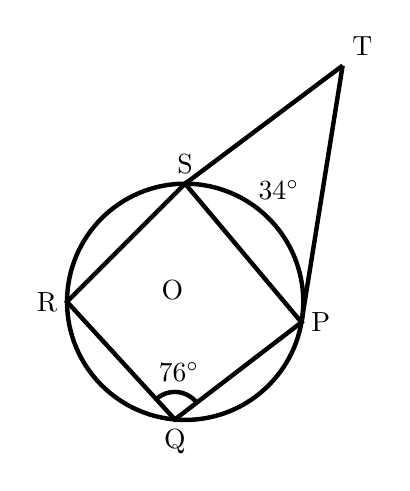
\begin{tikzpicture}

% Define radius
\def\r{1.5}

% Center O
\coordinate (O) at (0,0);

% Points on circle
\coordinate (R) at (180:\r);
\coordinate (S) at (90:\r);
\coordinate (P) at (-10:\r);
\coordinate (Q) at (265:\r);

% External point T
\coordinate (T) at (2,3);

% Draw circle
\draw[ultra thick] (O) circle (\r);

% Draw quadrilateral RSPQ
\draw[ultra thick] (R) -- (S) -- (P) -- (Q) -- cycle;

% Draw lines to T
\draw[ultra thick] (S) -- (T);
\draw[ultra thick] (P) -- (T);

% Labels for points
\node[left] at (R) {R};
\node[above] at (S) {S};
\node[above right] at (T) {T};
\node[right] at (P) {P};
\node[below] at (Q) {Q};
\node[above left] at (0.1,-0.1) {O};

% Calculate angles for the arc at Q (angle RQP = 76°)
\pgfmathsetmacro{\angQtoR}{atan2(0-\r*sin(265), -\r-\r*cos(265))}
\pgfmathsetmacro{\angQtoP}{atan2(\r*sin(-10)-\r*sin(265), \r*cos(-10)-\r*cos(265))}

% Draw 76° angle arc at Q (angle RQP)
\draw[ultra thick] ($(Q)+(\angQtoR:0.35)$) arc (\angQtoR:\angQtoP:0.35);
\node at ($(Q)+({(\angQtoR+\angQtoP)/2}:0.6)$) {$76^{\circ}$};

% Draw 34° on arc SP (on circle perimeter)
\node at (50:\r+0.35) {$34^{\circ}$};

\end{tikzpicture}
\end{document}